\section{Syntax der Aussagenlogik}
%Zur Darstellung von Aussagen in einer (für die Mathematik notwendigen) präzisen Struktur repräsentieren wir atomare Aussagen durch Großbuchstaben und Kombinationsmöglichkeiten von Aussagen durch spezielle Symbole. 
In diesem Abschnitt wird die Syntax von Aussagen exakt spezifiziert, damit ist festgelegt,
%welche mathematischen Zeichenketten Aussagen beschreiben und welche nicht. 
welche der aus den Grundelementen bildbaren Zeichenfolgen zulässig oder ``wohlgeformt'' sind und welche nicht.


\subsection{Alphabet der Aussagenlogik}
\begin{defi}Alphabet der Aussagenlogik\label{Definition 2.1}\end{defi}Das Alphabet der Aussagenlogik ist einer Menge von erlaubten Zeichen oder Symbolen und besteht aus:
\begin{itemize}
\item Aussagenvariablen: $p, q, r, s, t \ldots$
\item Junktoren: 
\begin{align*}
Negation  &\ \neg\\
Disjunktion &\ \vee\\  
Konjuktion &\ \wedge \\  
Implikation &\ \rightarrow\\      
Äquivalenz &\ \leftrightarrow\\ 
Exklusives \ Oder &\ \oplus\\  
Nor &\ \downarrow\\   
Nand &\ \uparrow\\
\end{align*}
\item Konstanten: $true$ und $false$\cite{Schenke}
\item Hilfssymbolen: $(,)$ 
\end{itemize}

\subsection{Syntax aussagenlogischer Formeln}
Die folgende Regeln bestimmt welche Zeichenketten, die von dem oberem Alphabet gebildet werden, wohlgeformte Ausdrücke (Formeln) sind, z.B während $(p \rightarrow q)$ eine aussagenlogische Formel ist, ist die $(\wedge p) q \vee)$ keine aussagenlogische Formel.
\begin{defi}\label{Definition 2.1} Formationsregeln\end{defi}
\begin{enumerate}
\item \label{formationsregeln_1}eine Aussagenvariable (atomare Aussage) ist eine Formel.
\item \label{formationsregeln_2}ist $A$ eine aussagenlogische Formel, dann ist auch $\neg A$ eine aussagenlogische Formel.
\item \label{formationsregeln_3}sind $A$ und $B$ aussagenlogische Formeln, dann sind
\begin{enumerate}
\item \label{formationsregeln_3_1}$(A \wedge B)$  
\item \label{formationsregeln_3_2} $(A \vee B)$  
\item $(A \rightarrow B)$   
\item $(A \leftrightarrow B)$      
\item $(A  \oplus B)$      
\item $(A \downarrow B)$      
\item $(A \uparrow B)$   
\end{enumerate}
ebenfalls aussagenlogische Formeln
\item \label{formationsregeln_4}Ein Ausdruck ist nur dann eine aussagenlogische Formel, wenn er durch Anwendung der oben­stehenden Regeln konstruiert werden kann.
\end{enumerate}

Um nachzuweisen, dass bestimmte Zeichenketten  keine wohlgeformten Formel sind, kann man auch beweisen, dass wohlgeformte Formel bestimmte Eigenschaften haben müssen. Wenn diese Zeichenkette eine dieser Eigenschaften nicht
erfüllt, so kann sie auch keine Formel sein.
\begin{bem}\label{AussagenEigenschaften}\cite{Dreiseitl}\end{bem} 
Solche Eigenschaften von Formeln sind etwa:
\begin{itemize}
\item Es gibt ebenso viele öffnende wie schließende Klammern,
\item links und rechts von jedem der Junktoren $\wedge$ und $\vee$ steht eine Formel,
\item eine Formel endet nie mit einem Junktor.
\end{itemize}

\begin{ex}\label{Beispiel 2.1}\end{ex}
Seien $p$, $q$ aussagenlogische Formeln. 
%(¬(p ∧ q) ⇒ (q∨¬q))
Die Zeichenkette $\neg(p \wedge q)$ ist eine Formel, da diese aus den Bildungsregeln \eqref{formationsregeln_1},\eqref{formationsregeln_3_1} und \eqref{formationsregeln_2}  zusammengesetzt werden können.

%((p ∧ ∨q))
Die Zeichenkette $((p \wedge \vee q))$ ist keine Formel, da $\vee q$ (rechts von $p \wedge$) und auch $p \wedge$ (links von $\vee q$) keine Formeln sind.\cite{Dreiseitl}


\subsection{Bindungskonventionen} \label{subsec:Bindungskonventionen}
Die Klammern um die Ausdrücke sind wichtig, weil durch sie die Reihenfolge der semantischen Auswertung geregelt wird, z.B Die Formel $(p \vee q) \wedge r$ wird anders ausgewertet als $p \vee (q \wedge r)$. Da viele Klammern Formeln unübersichtlich werden lassen, vereinbart man analog wie in der elementaren Arithmetik ``Punktrechnung geht vor Strichrechnung'' die folgende Bindungsregeln(von hoch nach niedrig):
\begin{align*}
\neg\\
\wedge, \uparrow\\
\vee, \downarrow\\
\rightarrow\\
\leftrightarrow, \oplus
\end{align*}

%Zusätzliche Klammern können immer verwendet werden, um eine Formel zu verdeutlichen: $(p \vee q) \wedge (q \vee r)$. Die Booleschen Operatoren $\wedge$, $\vee$, $\leftrightarrow$, $\oplus$ sind assoziativ. Daher wird man häufig Klammern in Formeln auslassen, in denen diese Operatoren wiederholt vorkommen: $p \vee q \vee r \vee s$. Beachtet man, dass $\rightarrow$, $\downarrow$, $\uparrow$ nicht assoziativ sind. Daher müssen Klammern verwendet werden, um Verwechslungen zu vermeiden. Obwohl angenommen wird, dass der Implikationsoperator rechts assoziativ ist, so dass $p \rightarrow q \rightarrow r$ eindeutig $p \rightarrow (q \rightarrow r)$ bedeutet, schreibt man die Formel mit Klammern, um eine Verwechslung mit $(p \rightarrow q) \rightarrow r$ zu vermeiden.


\subsection{Baum-Notation von Formeln}
Es ist oft vorteilhaft, sich die Struktur einer Formel $A$ (wie sie durch ihre Unterformeln aufgebaut ist) als einen Syntax-Baum mit Wurzel vorzustellen, dessen Blätter mit den atomaren Aussagen von $A$ und dessen innere Knoten mit geeigneten Junktoren markiert sind. Dabei stimmt die Stelligkeit des markierenden Junktors mit der Anzahl der Kinder überein.
%
%\begin{itemize}
%\item	Eine Formel ist ein mit einer $\neg$ gekennzeichneter Knoten mit einem einzelnen Kind, das eine Formel ist.
%\item	Eine Formel ist ein durch einen der binären Operatoren beschrifteter Knoten mit zwei Kindern, die beide Formeln sind.
%\end{itemize}
%
%%• Eine Formel ist ein Knoten, der mit einem ¬ gekennzeichnet, dann einen einzelnen Kind, das auch eine Formel ist, hat. 
%%• Eine Formel ist ein Knoten, der durch einen der binären Operatoren beschriftet, dann zwei Kindern, die beide auch Formeln sind, hat.

\begin{defi}Formeln als Bäume\label{Definition 2.2}\cite{Ben-Ari} \end{defi}Eine Formel in der Aussagenlogik ist ein rekursiv definierter Baum:
\begin{enumerate}
\item Eine Formel ist ein Blatt, das durch eine atomare Aussage gekennzeichnet ist.
\item Eine Formel ist ein mit einer $\neg$ gekennzeichneter Knoten mit einem einzelnen Kind, das eine Formel ist.
\item Eine Formel ist ein durch einen der binären Operatoren beschrifteter Knoten mit zwei Kindern, die beide Formeln sind.
\end{enumerate}
Abbildung \ref{Abb. 2.1} zeigt Baum-Notation von $p \rightarrow p \leftrightarrow \neg p \rightarrow \neg q $:
\begin {figure}[h]
\begin{center}
\definecolor{ududff}{rgb}{0.30196078431372547,0.30196078431372547,1}
\definecolor{uuuuuu}{rgb}{0,0,0}
\begin{tikzpicture}[line cap=round,line join=round,>=triangle 45,x=1cm,y=1cm]

\clip(-3.5,-6.5) rectangle (3.38,0.68);
\draw [line width=1pt] (0,0)-- (-2,-2);
\draw [line width=1pt] (0,0)-- (2,-2);
\draw [line width=1pt] (-2,-2.5)-- (-3,-4);
\draw [line width=1pt] (-2,-2.5)-- (-1,-4);
\draw [line width=1pt] (2,-2.5)-- (1,-4);
\draw [line width=1pt] (2,-2.5)-- (3,-4);
\draw [line width=1pt] (1,-4.5)-- (1,-6);
\draw [line width=1pt] (3,-4.5)-- (3,-6);
\begin{small}
\draw[color=uuuuuu] (0,0.33) node {$\leftrightarrow$};
\draw[color=uuuuuu] (-2,-2.25) node {$\rightarrow$};
\draw[color=uuuuuu] (2,-2.25) node {$\rightarrow$};;
\draw[color=uuuuuu] (-3,-4.25) node {$p$};
\draw[color=uuuuuu] (-1,-4.25) node {$q$};
\draw[color=uuuuuu] (1,-4.25) node {$\neg$};
\draw[color=uuuuuu] (3,-4.25) node {$\neg$};
\draw[color=uuuuuu] (1,-6.25) node {$p$};
\draw[color=uuuuuu] (3,-6.25) node {$q$};
\end{small}
\end{tikzpicture}
\end{center}
\caption[Beispiel Konstruktion für eine Formel]{Formel $p \rightarrow p \leftrightarrow \neg p \rightarrow \neg q $ ist ein Baum}	
\label{Abb. 2.1}
\end{figure}

\begin{bem}\label{FormelAlsString}\end{bem}
So wie man Ausdrücke als Strings schreibt (lineare Folgen von Symbolen), kann man Formeln als Strings schreiben. Die einer Formel zugeordnete Zeichenfolge kann durch eine Inorder-Traversierung des Baums erhalten werden.


\subsection{Operator-Notation}\label{subsec:Notation}
Die Bücher über mathematische Logik benutzen eine stark variierende Notation für die Booleschen Operatoren. Außerdem erscheinen die Operatoren in Programmiersprachen mit einer anderen Notation als es in Mathematikbüchern verwendet wird. Folgende Tabelle zeigt einige dieser alternativen Notationen.

\begin{table}[h]

			\begin{center}
			\begin{tabular}{ccc}
			\hline
			\textbf{Junktor} & \textbf{Literatur} & \textbf{Java}\\
			\hline
			\hline
			$\neg$ &$\sim$& !\\
			\hline
			$\wedge$  & \& & \&, \&\&  \\
			\hline
			$\vee$ &  & |,||\\
			\hline
			$\rightarrow$  & $\supset,\Rightarrow$ & \\
			\hline
			$\leftrightarrow$ & $\equiv,\Leftrightarrow$ & \\
			\hline
			$\oplus$ &$\not\equiv$ &$\mbox{\textasciicircum}$ \\
			\hline
			\end{tabular}
			\end{center}
			\caption[Notationen der Booleschen Operatoren]{Alternative Notationen\cite{Ben-Ari}}
			\label{Notationen}
			\end{table}
			
\subsection{Eine formale Grammatik für Formeln}\label{subsec:FormelGrammatik}

%Dieser Unterabschnitt setzt Vertrautheit mit formalen Grammatiken voraus. Anstatt Formeln als Bäume zu definieren, können sie als Strings definiert werden, die eine kontextfreie formale Grammatik generieren.

Dieser Unterabschnitt setzt Vertrautheit mit formalen Grammatiken voraus. Anstatt Formeln als Bäume zu definieren, können sie als Strings, die über einer kontextfreien formalen Grammatik generiert werden, definiert werden.

\begin{defi} \label{Definition 2.13}Kontextfreien Grammatik für Formel \end{defi} Formeln in der Aussagenlogik werden aus der kontextfreien Grammatik abgeleitet, deren Terminals sind \cite{Ben-Ari}:
\begin{itemize}
\item  Eine unbegrenzte Menge von Symbolen $\mathcal{P}$, die atomare Propositionen heißen.
\item  Die Booleschen Operatoren in Definition \ref{Definition 2.1}.
\end{itemize}
Die Produktionen der Grammatik sind:
\begin{align*}
fml &:: = p \ für \ jedes \ p \in  \mathcal{P}\\
fml &:: = \neg fml\\
fml &:: = fml \  op \ fml\\
op &:: = \vee | \wedge | \rightarrow  |\leftrightarrow | \oplus | \uparrow | \downarrow
\end{align*}


%Eine Formel ist ein Wort, das aus dem Nichtterminal $fml$ abgeleitet werden kann. Die Menge von allen Formeln, die von der Grammatik abgeleitet werden können, sind mit $\mathcal{F}$ bezeichnet. Ableitungen von Strings (Wörtern) in einer formalen Grammatik können als Bäume dargestellt werden (Hopcroft et al., 2006, Abschn. 4.3). Das durch eine Ableitung erzeugte Wort kann gelesen werden von den Blättern von links nach rechts.






















%\begin{ex} \label{Beispiel 2.14} \end{ex} Hier ist eine Herleitung der Formel p $\rightarrow$    q $\leftrightarrow$ $\neg$p $\rightarrow$   $\neg$q in der Aussagenlogik; Der Baum, der seine Ableitung darstellt, ist in Abb. \ref{Abb. 2.2} dargestellt.
%
%\begin{figure}[ !h] \centering												
% 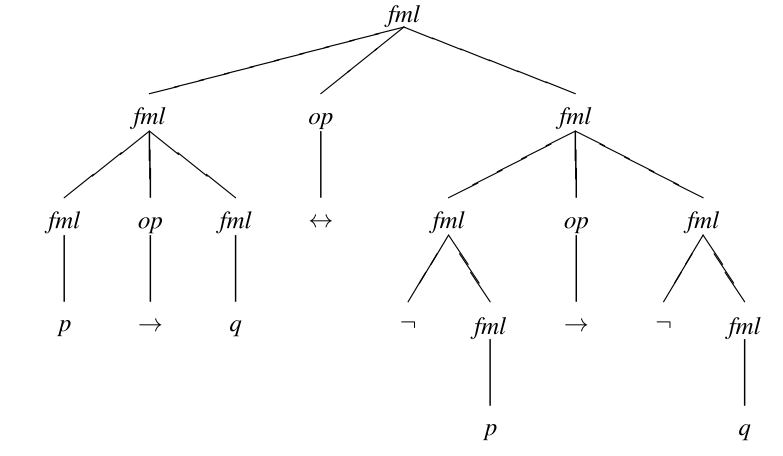
\includegraphics[width=1.0\textwidth]{A3}					
% \caption[Ableitungsbaum für p $\rightarrow$   q $\leftrightarrow$ $\neg$p $\rightarrow$  $\neg$q]{Derivation tree for p $\rightarrow$   q $\leftrightarrow$ $\neg$p $\rightarrow$  $\neg$q}					
% \label{Abb. 2.2} 
%\end{figure}
%
%\begin{align*}
%&fml\\
%&fml \  op \ fml\\
%&fml \leftrightarrow fml\\
%&fml \  op \  fml \leftrightarrow fml\\
%&fml \rightarrow fml \leftrightarrow fml\\
%&p \rightarrow fml \leftrightarrow fml\\
%&p \rightarrow q \leftrightarrow fml\\
%&p \rightarrow q \leftrightarrow fml  \  op \  fml\\
%&p \rightarrow q \leftrightarrow fml \rightarrow fml\\
%&p \rightarrow q \leftrightarrow \neg fml \rightarrow fml\\
%&p \rightarrow q \leftrightarrow \neg p \rightarrow fml\\
%&p \rightarrow q \leftrightarrow \neg p \rightarrow \neg q
%\end{align*}
%
%
%
%%\begin{figure}[ !h] \centering												
%% 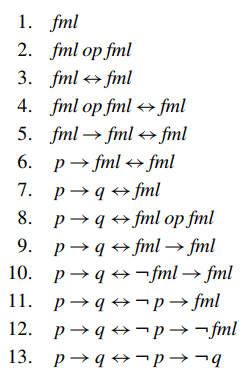
\includegraphics[width=0.3\textwidth]{A0}									
%% \label{Abb. A0}
%%\end{figure}
%
%
%Die in Abschn. \ref{sssec:num1} kann zur Auflösung von Mehrdeutigkeiten verwendet werden. Wir können die Grammatik ändern, um Klammern einzuführen: 
%\begin{align*}
%fml &:: = (\neg \  fml)\\
%fml &:: = (fml \  op \  fml)
%\end{align*}
%und dann die Präzedenz verwenden, um ihre Anzahl zu reduzieren.
%
